%\documentclass[conference]{IEEEtran}
\documentclass[10pt,conference,anonymous]{IEEEtran}
\IEEEoverridecommandlockouts

%% Marcelo added this
\makeatletter
\renewcommand\footnoterule{%
  \kern-3\p@
  \hrule\@width.4\columnwidth
  \kern2.6\p@}
  \makeatother




\usepackage{inconsolata}
\usepackage{listings}

\lstset{language=Java,
basicstyle=\ttfamily\scriptsize,
%basicstyle=\ttfamily,
keywordstyle=\color{javapurple}\bfseries,
stringstyle=\color{pblue},
commentstyle=\color{javagreen},
morecomment=[s][\color{javadocblue}]{/**}{*/},
morecomment=[s][\color{gray}]{@}{\ },
numbers=left,
numberstyle=\tiny\color{black},
stepnumber=2,
numbersep=8pt,
tabsize=4,
showspaces=false,
showstringspaces=false,
breaklines=true,}

%%%%%%%%%%%%%%%%%%%%%%%%%%%%%%%%%%




\usepackage{adjustbox} % ajustar tabela ao tamanho da pagina

\usepackage{tikz}
\usetikzlibrary{matrix,fit,shapes,calc,positioning,shadows,arrows,shapes,backgrounds,decorations.markings,fadings}
\usepackage{graphicx}
\usepackage{multirow}
\usepackage[caption=false, font=footnotesize]{subfig}
\usepackage{wrapfig}
\usepackage{enumitem}
\usepackage{url}
%% helpers
\newcommand{\js}{JS}
\newcommand{\javascript}{JavaScript}
\newcommand{\es}{ES}
\newcommand{\ecmascript}{\es{}}
\newcommand{\tname}{TNAME}
\newcommand{\Comment}[1]{}
\newcommand{\numsubjects}{5}
\newcommand{\etal}{and colleagues'}
\newcommand{\ie}{i.e.}
\newcommand{\eg}{e.g.}
\newcommand{\cmark}{\ding{51}}%
\newcommand{\xmark}{{\color{red}\ding{55}}}%
\newcommand{\pGoodGood}{$\mathit{P}${\small\cmark\!\cmark}}%
\newcommand{\pGoodBad}{$\mathit{P}${\small\cmark\!\xmark}}%
\newcommand{\pBadDontCare}{$\mathit{P_?}$}%
\newcommand{\sfl}{SFL\xspace}
\newcommand{\ddg}{DDG\xspace}
\newcommand{\totfiles}{$\sim$38K}

%% annotations
\newif\ifdraftmode
%% Comment or uncomment the \draftmodetrue line.
\draftmodetrue
\ifdraftmode
 \newcommand{\Fix}[1]{\textbf{[[}{\color{red} #1}\textbf{]]}}
 \newcommand{\Mar}[1]{\textbf{[[Marcelo: }{\color{magenta} #1}\textbf{]]}}
 \newcommand{\Igor}[1]{\textbf{[[Igor: }{\color{blue} #1}\textbf{]]}}
 \newcommand{\note}[1]{\todo[inline,color=red!30,caption={}]{#1}}
\else
 \newcommand{\Fix}[1]{\relax}
 \newcommand{\Mar}[1]{\relax}
 \newcommand{\Igor}[1]{\relax}
 \newcommand{\note}[1]{\relax}
\fi

% For submitted version only.
\pagenumbering{arabic}

% Uncomment this if you need more space
%% \makeatletter
%% \def\@copyrightspace{\enlargethispage{-10pt}\relax}
%% \makeatother

\newcommand{\codesize}{\small}
\newcommand{\CodeIn}[1]{\mcodeid{#1}}
\newcommand{\CodeInM}[1]{\mcodeid{#1}}
% \|name| or \mathid{name} denotes identifiers and slots in formulas
\def\|#1|{\mathid{#1}}
\newcommand{\mathid}[1]{\ensuremath{\mathit{#1}}}
% \<name> or \codeid{name} denotes computer code identifiers
\def\<#1>{\codeid{#1}}
\newcommand{\codeid}[1]{\ifmmode{\mbox{\codesize\ttfamily{#1}}}\else{\codesize\ttfamily #1}\fi}
\def\<#1>{\mcodeid{#1}}
\newcommand{\mcodeid}[1]{\mbox{\codesize\ttfamily{#1}}}

%% thumbs up down
\newcommand*{\RightThumbsUpAux}[1]{%
  \begingroup
    \sbox0{Ag}%
    \raisebox{-\dp0}{%
      \includegraphics[{%
        height=\dimexpr\dp0+\ht0\relax,
        #1%
      }]{thumbsup.pdf}%
    }%
  \endgroup
}
\newcommand*{\RightThumbsUp}{%
  \RightThumbsUpAux{}%
}
\newcommand*{\RightThumbsDown}{%
  \RightThumbsUpAux{origin=c,angle=180}%
}
\newcommand*{\LeftThumbsUp}{%
  \scalebox{-1}[1]{\RightThumbsUp}%
}
\newcommand*{\LeftThumbsDown}{%
  \scalebox{-1}[1]{\RightThumbsDown}%
}

\newcommand{\checkm}{Y}
\newcommand{\crossmark}{N}
%\begin{wraptable}[20]{t}[0pt]{0.5\textwidth}

\newcommand{\totalTestFiles}{38,369}
\newcommand{\totalTestFilesCompileInAll}{35,939}
\newcommand{\totalTestFilesPassInAll}{24,493}
\newcommand{\nofuzzAll}{209}
\newcommand{\nofuzzBugs}{\Fix{XX}}
\newcommand{\nofuzzDuplicates}{63}
\newcommand{\nofuzzFalsePositives}{24}
\newcommand{\nofuzzHITotal}{177}
\newcommand{\nofuzzLOTotal}{32}
\newcommand{\nofuzzTotalFiles}{977} % conflicting files
\newcommand{\nofuzzFilesHI}{940} % conflicting files HI
\newcommand{\nofuzzFilesLO}{37} % conflicting files LO

\newcommand{\nofuzzBucketsBugsHI}{\Fix{124}} % buckets reported (including dups)
\newcommand{\nofuzzBucketsBugsLO}{\Fix{11}} % buckets reported
\newcommand{\nofuzzDupsHI}{\Fix{X}}
\newcommand{\nofuzzDupsLO}{\Fix{Y}}

% continue updating bugs table
\newcommand{\tableBugsNum}{\Fix{26}}

%% anonymize

\newcommand{\anonym}[1]{{\tiny\colorbox{black}{#1}}}

%% names
\newcommand{\radamsa}{radamsa}
\newcommand{\quickfuzz}{quickfuzz}

\newcommand{\jsc}{JavaScriptCore}
\newcommand{\veight}{V8}
\newcommand{\chakra}{Chakra}
\newcommand{\smonkey}{SpiderMonkey}
\newcommand{\jerry}{JerryScript}

\newcommand{\lo}{lo}
\newcommand{\hi}{hi}


\begin{document}

%Should I Fuzz my Inputs or Improve my Tests? 
\title{Differential Testing Runtime Engines--Lessons Learned from the
  JavaScript Domain}

%% \author{
%% \IEEEauthorblockN{Sabrina Souto}
%% \IEEEauthorblockA{State University of Para\'iba\\
%% Para\'iba, Brazil\\
%% sabrinadfs@gmail.com}
%% \and
%% \IEEEauthorblockN{Marcelo d'Amorim}
%% \IEEEauthorblockA{Federal University of Pernambuco\\
%%   Pernambuco, Brazil\\
%%   damorim@cin.ufpe.br}
%% \and
%% \IEEEauthorblockN{Rohit Gheyi}
%% \IEEEauthorblockA{Federal University of Campina Grande\\
%%   Para\'iba, Brazil\\
%%   rohit@dsc.ufcg.edu.br}
%% }

\maketitle

%% page numbering -M
\thispagestyle{plain}
\pagestyle{plain}

%% JavaScript (\js{}) is a popular programming language for the
%% web. Finding errors in JS runtime engines is an important problem.
\begin{abstract}
This paper assesses the impact of Differential Testing (DT) to find
functional bugs in JS engines. This is an important problem given the
importance of JS today. DT has shown successful in finding bugs in
compilers and runtimes, but has not been thoroughly explored in this
important domain. Our study \Fix{...}
\end{abstract}

\begin{IEEEkeywords}
...
\end{IEEEkeywords}

\section{Introduction}

JavaScript (\js{}) is today one of the most popular programming
languages for the web~\cite{business-insider,stackify}. The interest
of the community for the language encourages constant improvements in
its specification and implementations. It is natural to expect that
such improvements will entail sensible changes in runtime
engines~\cite{kangax}; changes that could lead to errors. Finding bugs
on JS engines is an important problem. 

Differential testing~\cite{Brumley-etal-ss07} (DT) is a popular
approach that has been applied in a variety of contexts to find
functional bugs in
software~\cite{Yang-etal-pldi11,Chen-etal-fse2015,Argyros-etla-ccs16,Chen-etal-pldi16,petsios-etal-sp2017,SivakornAPKJ17}. It
automates test generation in scenarios where multiple implementations
of a system exist. DT leverages the diversity across system's
implementations to detect anomalous behavior. For example, Mozilla
runs JS files--created with the grammar-based fuzzer
jsfunfuzz~\cite{jsfunfuzz}--against different configurations of their
SpiderMonkey engine~\cite{jsfunfuzz-mozilla-bug} to find discrepancies
across configurations. They use this technique since 2002 and have
been able to find over 270 bugs since
then~\cite{jsfunfuzz-at-mozilla}, some of which are security bugs.
Cross-engine differential testing checks correctness by comparing the
output produced by \emph{different} engines on a given
input~\cite{patra2016learning}. The availability on the web of public
implementations of JS engines (see Table~\ref{tab:engines}) and test
suites makes this bug-finding approach very appealing.

%% WHAT WE DID
This paper reports the results of a study we conducted to (i) assess
the reliability of existing JS engines and to (ii) evaluate the
importance of different factors when using DT for bug finding. More
precisely, we analyzed the impact of two orthogonal factors in the use
of DT: test mining and fuzzing. The first dimension, test mining,
considers the effect that \js{} test files mined from the repository
of a given open-source engine have in detecting functional bugs in
other engines. The second dimension, fuzzing, considers the impact of
fuzzing the mined files in bug detection.
%% WHAT WE FOUND
To sum, we found that \Fix{...}

%% LIST OF CONTRIBUTIONS
This paper makes the following contributions \Fix{...}

\section{ES6 design}
\label{sec:es6-design}
The EcmaScript is a language specification maintained by 
a committee called TC39 (Technical Committee) that follows 
standard rules proposed by ISO/ETC JTC 1 - 
Information Technology since 1996~\cite{es6-website}.
Every year, a new version of EcmaScript (the latest version is ES2017) adds
new features and minor fixes for the language. \Fix{discutir mais
  sobre isso}

\Mar{what is that exactly? can we cite? is that only spec or actually
  code as most of java.* libraries.}  \Igor{seems like an API. They
  define the language behavior; grammar; values to static variables;
  the methods for each "class"(Object)...  These irregularities
  appears on engine implementation, maybe an wrong if statement and so
  on.} \Mar{Igor, avoid general discussion like $\leftarrow$this. look for
  explanation in some forum/tutorial and explain **when** you
  undertand the JS ecosystem design and can explain with confidence.}

\Mar{explain what is an **acceptable** incompatibilities. cite example
bug reports.}
\Igor{For example, the latest version of ES specs~\cite{es6-spec} describes that
the function \CodeIn{Number.toPrecision(precision)}, in general,
if precision is defined the method returns a String 
containing the Number value represented either 
in decimal exponential notation or in decimal 
fixed notation~\cite{es6-toPrecision}. The Number object uses a 
property that the specification describes as approximately so when we use 
toPrecision with a bigger precision, the values of each engine may vary, this
could be considered as a case of incompatibility by engine
design.}\Mar{I don't understand the example very well and don't understand the
  relationship with HI/LO.}

\subsection{Randomness and Undefined Behavior}

\Mar{answer from C. Holler. Think through this...}

1) The stack depth in JS is often close to the real (native) C stack depth, nevertheless observable by JS through recursion. This causes differential behavior even on the same engine when JITs are enabled or disabled, as the stack frame sizes vary. LangFuzz in particular produces a lot of recursions and hits these problems even more often than jsfunfuzz.

2) JS has some "undefined behavior", such as the enumeration order of object properties in certain cases. In our engine, we have an --enable-more-deterministic mode (build option) to solve some of these issues.

3) JS naturally has some observable differential behavior in global objects, e.g. Math.random, Date, etc. These can often be mocked to solve these issues, but fuzzers can be surprisingly effective to find more of these sources or even get the old objects back somehow.

\section{Infrastructure}
\label{sec:design}


%\begin{wrapfigure}[10]{r}[0pt]{0.45\textwidth}
\begin{figure}[t]
  \centering
%  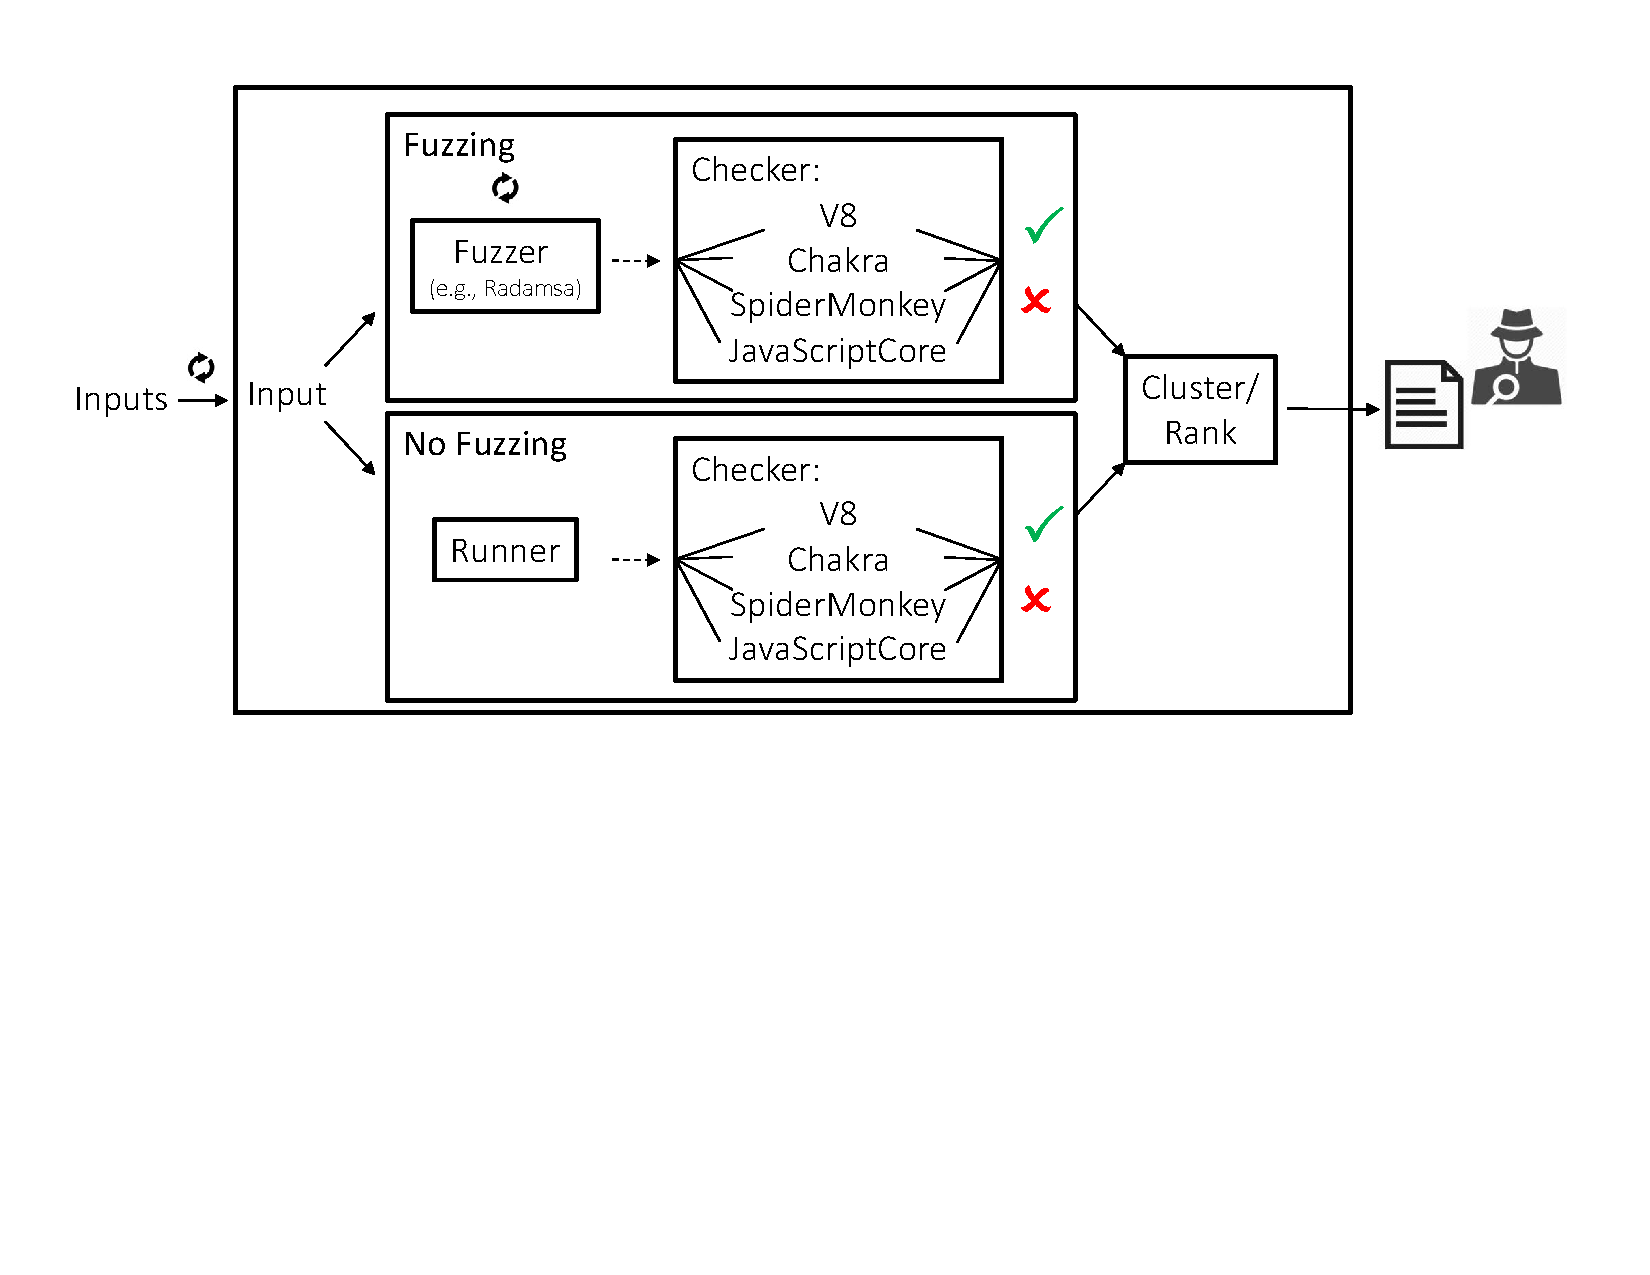
\includegraphics[trim=20 350 200
%    0,clip,width=0.35\textwidth]{google-awards-workflow}
  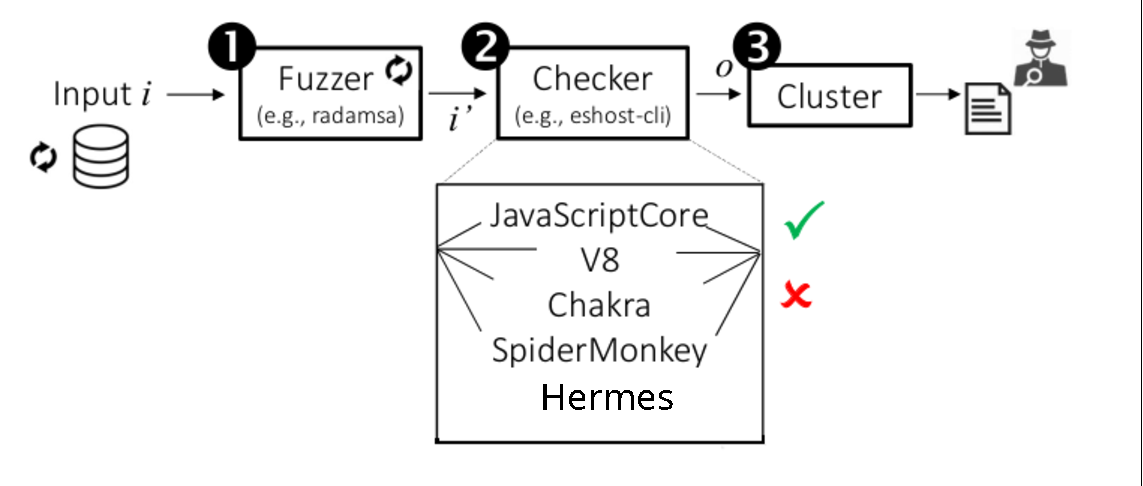
\includegraphics[trim=0 350 0 0,clip,width=0.65\textwidth]{diff-testing-runtimes}
  \caption{\label{fig:workflow}Infrastructure.}
\end{figure}

Figure~\ref{fig:workflow} illustrates the infrastructure we used in
this study.  The bug-finding process takes on input JS files from
regression test suites of various JS engines and generates warnings on
output. Boxes in the figure denote encapsulation; arrowed lines
indicate data flow. The cycle icons denote repetition--the leftmost
icon indicates that each file in the input list will be analyzed in
separate whereas the rightmost icon shows that a single file will be
fuzzed multiple times. The bug-finding process works as follows.
Considering the case where fuzzing is not selected, the oracle checks
whether or not the output produced for the input file is consistent
across all engine implementations. In case the test passes in all
engines or fails in all engines (\ie{}, the output is consistent), the
infrastructure discards the test. Otherwise, it considers the input as
potentially fault-revealing; hence interesting for human
inspection. We used the open-source eshost-cli
project~\cite{eshost-cli} for that. Microsoft uses eshost-cli to check
functional discrepancies in the Chakra JS engine. Considering the case
where fuzzing~\cite{fuzz-testing-history} is selected, new inputs are
obtained from a given input using some off-the-shelf fuzzer. The
workflow with fuzzing is similar to the workflow without fuzzing. In
this case, however, the checker can produce multiple warnings for a
given input. Several fuzzing methods have been proposed in the past,
varying with respect to how new inputs are
generated~\cite{afl,honggfuzz,grammarinator,jsfunfuzz,radamsa}.
Section~\ref{sec:objects:fuzzers} describes the fuzzers we selected.



The infrastructure outputs a list of warnings for human inspection.
To reduce the number of false alarms, we clustered warnings in two
groups, reflecting their likelihood to manifest a real bug. Warnings
in the HI group are associated with the cases where the anomaly has
been detected in during the execution of test code or its close
%% the rationale we provide is related to the above; not crashes
neighborhood. The rationale is that the test in this group executed
without violating any internal checks of the API. In constrast,
warnings in the LO group reflect the cases where the anomaly was
observed during the execution of functions from standard JS libraries\Fix{check}.
  We found that different engines often check pre-conditions of
those functions differently. It can happen, for example, that one
engine enforces a weaker pre-condition compared to another.
% \Mar{why is that?
% that should not happen if the spec was fully documented and engines
% properly implemented those checks. Explain and give example.}
%% \Igor{these cases happen because the specification describes how a function
%% should work, however the internal implementation is defined by the
%% engine developers}\Mar{If you confirm that there is no code in specs
%%   (see comment above), what would be those abstract
%%   functions/interfaces that you mentioned to me the other day?}.
In those cases, our infrastructure would observe a discrepancy that is more likely to
be associated with a bug in the fuzzed test; not the code. Although
we did find real bugs from warnings in the LO group, the proportion
was much lower compared to the HI group--only \Fix{12\%} of the reals bugs
we found originated from the LO category.

% I think this will make the definition of HI/LO weaker. We can
% elaborate this later. for example, in the evaluation.
%% \Igor{In addiction, we inserts in LO groups tests that generates a timeout warning
%% due the capacity of a fuzzer add an infinite repetition statement. We expected that
%% each test process can running utmost 5 seconds, if exceed this condition we stop 
%% the process and add a output message of a TIMEOUT error.}

\Igor{
  We defined if a warning is in HI or LO group according to console output.
  The error stream in the output shows relevant informations that we can 
  process. The Figure~\ref{fig:error-output} shows examples of HI and LO warning
  outputs based on the stream output came from Chakra engine. 
  % The error message shows informations related to the assertion code (see at line 2) 
  % that thows an Error exception. This case was considered as HI groups and after 
  % several discussion and specification analysis we reported as a true positive example (see \cite{bug4978}).
}\Mar{igor, first add the real example then draft the discussion}


% \begin{figure}[h!]
%   \centering
%   \scriptsize
%   \lstset{escapeinside={@}{@},
%     numbers=left,xleftmargin=1em,frame=single,framexleftmargin=0.5em,
%     basicstyle=\ttfamily\scriptsize, boxpos=c,
%     numberstyle=\tiny,
%     morekeywords={assertEq, var, yield, in, function, 
%     typeof, return, throw, new, Error, if},
%   }
% \begin{lstlisting}

% \end{lstlisting}
% \normalsize
% \caption{Warning captured as HI priority.}
% \label{fig:hi-priority}
% \end{figure}

% bug high console output
% This a case of a warning reported as HI priority, the Figure~\ref{} shows
% the output console of V8 engine. We consider this case as a HI group due 
% the fail by assertion, defined at line 2 as \CodeIn{throw new Error("Test failed");}

% \begin{figure}[h!]
%   \centering
%   \scriptsize
%   \lstset{escapeinside={@}{@},
%     numbers=left,xleftmargin=1em,frame=single,framexleftmargin=0.5em,
%     basicstyle=\ttfamily\scriptsize, boxpos=c,
%     numberstyle=\tiny,
%     morekeywords={assertEq, var, yield, in, function, 
%     typeof, return, throw, new, Error, if},
%   }
% \begin{lstlisting}
% function test() {
%   var buffer = new ArrayBuffer(64);
%   var view = new DataView(buffer);
%   view.setInt8 (0, 0x80);
%   -return view.getInt8(0) === -0x80;
  
%   // radamsa fuzzing
%   +return view.getInt8(-1770523502845470856862803727694) === -0x80;
%   }
  
%   if (!test())
%       throw new Error("Test Failed");
% \end{lstlisting}
% \normalsize
% \caption{Warning captured as HI priority.}
% \label{fig:hi-priority}
% \end{figure}

% no-bug low console output
% \begin{figure}[h!]
%   \centering
%   \scriptsize
%   \lstset{escapeinside={@}{@},
%     numbers=left,xleftmargin=1em,frame=single,framexleftmargin=0.5em,
%     basicstyle=\ttfamily\scriptsize, boxpos=c,
%     numberstyle=\tiny,
%     morekeywords={assertEq, var, yield, in, function, 
%     typeof, return, throw, new, Error, if},
%   }
%   \begin{lstlisting}
% \end{lstlisting}
% \normalsize
% \caption{Warning captured as HI priority.}
% \label{fig:lo-priority}
% \end{figure}

%% \Mar{can we detect dups mining issue trackers?}
%% \Igor{
%%   acho que encontrar duplicatas seria um estudo a parte, devido a linguagem natural.
%%   Tenho umas consideracoes:
%%   \begin{itemize}
%%     \item warning HI possui a msg "Error: Test Failed", nao tem como buscar algo com isso, 
%%     se for pegar a linha que falhou, provavelmente vai mostrar a linha onde o assert se encontra.
%%     \item warning LO: podemos tentar conseguir buscar pelo output/funcao que falhou,
%%     \item O fuzzinator tem algo similar (dei uma olhada rapida, nao eh complicado)
%%   \end{itemize}
%% }\Mar{i think this is not the proper place to
%%   add this. discuss this with me.}

\section{Objects of Study}
\label{sec:methodology}

This section discusses the objects we used in our study.

\subsection{Engines}
\label{sec:methodology:engines}~We selected 
JS engines according to the following criteria.

\begin{itemize}
\item Released latest version after Jan 1, 2018
\item Contains more than 1K starts, if on GitHub  
\item Uses a public issue tracker
\end{itemize}  

We look for highly-maintained (as per the first criterion) and popular
(as per the second criterion) projects. As we wanted to report bugs,
we also looked for project with public issue trackers.
It is worth noting that we used
GoogleChromeLab's JSVU~\cite{jsvu} to automatically install and configure versions of
different JS engines in our host environment. This is important as we
aim to use the most recent stable versions of each engine as to avoid
reporting old and already-fixed bugs to developers.

%% Table~\ref{tab:engines} shows the engines we selected in this
%% study. We made an exception to the second criterion with
%% XS~\cite{xs2018repo}. As the project is young, created in Oct 2017, we
%% thought there was insufficient time to obtain 1K stars for XS. We
%% still considered this project as it seems to be attracting interest
%% from the community\Fix{is this true?}

\begin{table}[t]
  \centering
  \caption{\label{tab:engines}Engines Analyzed.}
  \begin{tabular}{cccr}
    \toprule
    Group & Name & URL & \# Stars \\
    \midrule
    Apple & JavaScriptCore (WebKit) & \cite{jsc2018repo} & \multicolumn{1}{c}{-} \\
    Google & v8 & \cite{v82018repo} & 9800+ \\
    JerryScript & JerryScript & \cite{jerryscript2018repo} & 3100+ \\
    Microsoft & Chakra & \cite{chakra2018repo} & 7200+ \\
%    Moddable & XS & \cite{xs2018repo} & 140+ \\
    \midrule
    \multirow{2}{*}{Mozilla} & Rhino & \cite{rhino2018repo} & 1800+ \\
    & SpiderMonkey & \cite{spidermonkey2018repo} & \multicolumn{1}{c}{-} \\
   \bottomrule     
  \end{tabular}
\end{table}

\subsection{Seed JS files\label{sec:seeds}}~
We selected test files from several public projects from GitHub. We
looked for self-contained tests from JS engine projects, initially
using the GitHub REST API~\cite{github-rest-api}. We noticed that some
of the tests we found depend on external libraries, which not all
engines we use (see Section~\ref{sec:methodology:engines}) support. We
decided to discard those. For example, many tests we found required a
Node.js runtime~\cite{node} for execution. We considered the offical
TC-39~\cite{tc39-github} conformance test suite for the ECMA262
specification~\cite{ecmas262-spec}. Furthermore, we considered test
suites of three of the four engines mentioned in
Section~\ref{sec:methodology:engines} and four other engines.
Table~\ref{tab:test-suites} shows the JS sources we considered for
each of the selected projects. Overall, we found a total of
\totfiles{} JS files. It is worth noting that some test suites use
distinct frameworks for testing and require external libraries to run
their testing suites.  For these projects, we needed to make small
changes in the testing infrastructure to be able to run the tests
uniformly across all engines. More precisely, we needed to mock
functions, related to the test harness, which are only available to
certain engines.

\begin{table}[t]
  \centering
  \caption{\label{tab:test-suites}Test Suites. The sections of the
    table show, respectively, the TC-39 conformance test suite, suites
    from engines we analyzed, and other suites.}
  \begin{tabular}{ccr}
    \toprule
    Name & Source & \# JS files \\
    \midrule
    TC-39 (Test262) & \cite{ecma262-conformance-suite} & 45,144 \\
    \midrule
    Mozilla & \cite{mozilla} & 2,633 \\
    V8 & \cite{v8} & 64 \\
    WebKit & \cite{webkit} & 1,031 \\
    \midrule    
    Duktape & \cite{duktape} & 997 \\
    JerryScript & \cite{jerryscript} & 1,803 \\
    JSI & \cite{jsi} & 99 \\
    Tiny-js & \cite{tinyjs} & 44 \\    
    % Chakra & \cite{chakracore} & 2632 \\
    \midrule
     &  & 51,815 \\
   \bottomrule     
  \end{tabular}
\end{table}

% For example to run the JerryScript tests it was necessary 
% use the unit-test package to run it, but with our changes we added the assertion
% does not have an assertion in the test file
% \Fix{add code to explain}

\subsection{Fuzzers}
\label{sec:objects:fuzzers}

%% In the following, we describe the list of fuzzers we analyzed. We
%% initially considered generational grammar-based fuzzers and mutational
%% fuzzers.

Fuzzers are typically categorized in two main groups--those that build
inputs anew (generational) and those that modify existing inputs
(mutational). We used two black-box mutational
fuzzers\Comment{Radamsa~\cite{radamsa} and QuickFuzz~\cite{quickfuzz}}
in this study. In the following, we provide rationale for this
selection.

Generational fuzzers are typically grammar-based. These fuzzers
generate a new file using the grammar of the language whose inputs
should be fuzzed. Intuitively, those fuzzers implement a traversal of
the production rules of the input grammar to create syntax trees,
which are then pretty-printed. Consequently, this approach produces
inputs that are syntactically valid by construction.  We analyzed
three grammar-based fuzzers--Grammarinator~\cite{grammarinator},
jsfunfuzz~\cite{jsfunfuzz}, and
QuickFuzz~\cite{quickfuzz,grieco2016quickfuzz}.  Unfortunately, none
of those was effective out of the box. Given the bound limits we
defined on the number of inputs to generate and the exploration depth
of the syntax tree, we were unable to find discrepancies on the inputs
those tools generated. To sum, the tools produced a high percentage of
semantically-invalid inputs (\eg{}, \Fix{give one or two concrete
  examples--variable usage without definition?}) that we needed to
discard and the valid inputs manifested no discrepancies. For example,
we produced 100K inputs with Grammarinator and only \Fix{X} of those
were valid. With QuickFuzz, we were able to produce \Fix{Y, Y$>$Y?}
valid inputs as it contains some heuristics to circumvent violation of
certain type rules such as \Fix{variable used must be
  defined?}. Nonetheless, running those inputs in our infrastructure
we were unable to find discrepancies. Inpecting those inputs, we
realized that they reflected very simple scenarios.\Comment{ \Mar{are there
  weights associated with production rules besides the depth you can
  set?}} Although grammar-based fuzzers has been shown effective to
find real bugs\Fix{cite some jsfunfuzz bug reports}, generating
valid inputs is very time-consuming, especially for the context of
differential testing. For this reason, we did not consider those fuzzers.

%% Our
%% infrastructure supports any grammar fuzzer with a few
%% adjusts. However, we try to integrate several grammar-based fuzzers,
%% for example
%% and \Fix{others fuzzers} to
%% generate new JavaScript files based on grammar, but after several runs
%% it was observed that this approach was ineffective due the amount of
%% invalid files and/or files without discrepancies.
%% For example, if we
%% ran Grammarinator to generate 1K JS files ten times with a random seed
%% generation, we obtained \Fix{XX\%} of valid files. Checking in our
%% environment almost \Fix{XX\%} are js files that shows undefined
%% variables and due the differential testing in our environment all
%% engines will raise a SyntaxError and this approach was not relevant to
%% our experiment.

%% We initially considered used representatives of popular fuzzing approaches. For
%% random-based fuzzing we used Radamsa~\cite{radamsa}; for
%% coverage-based fuzzing we used
%% \Fix{AFL~\cite{afl}/libfuzzer~\cite{libfuzzer}?}, and for
%% generative-based fuzzing we used
%% \Fix{grammarinator,jsfunfuzz?}. Details on how these fuzzers work can
%% be found elsewhere~\cite{fuzz-bart}.

Mutational fuzzers can be either white-box or black-box. White-box
mutational fuzzers are typically coverage-based. American Fuzz Loop
(AFL)~\cite{afl} and libFuzzer~\cite{libfuzzer} are examples of this
kind of fuzzers. These fuzzers run tests inputs against instrumented
versions of the program under testing with the typical goal of finding
univeral errors like crashes and buffer overflows. The instrumentation
adds code to collect branch coverage and to monitor specific
properties\footnote{There are options in the clang toolchain to build
  programs with fuzzing instrumentation~\cite{libfuzzer}. clang
  provides several sanitizers for property
  checking~\cite{clang-documentation}.}. AFL use coverage to determine
inputs that uncover a new branch and deserve fuzzing whereas libFuzzer
uses evolutionary generation--it tries to minimize the distances to
still-uncovered branches of the program. AFL takes the instrumented
program binary (say, a JS engine) and one seed input to that program
(say, a JS program) and produces on output fault-revealing inputs, if
found. Considering our context of application, we needed to instrument
one runtime engine for fuzzing; we chose v8. Unfortunately, we found
that most of the inputs produced by AFL violate the JS
grammar. Furthermore, the fuzzing task can take daysfor a single seed
input and there is no simple way to guide the
exploration~\Fix{cite}. That happens because the fuzzer aims to
explore the entire decision tree induced from the engine's main
function, including the branches associated with the lexer and the
parser. For those reasons, coverage-based fuzzers were not considered
in this study. It is worth mentioning that Google mitigates that
problem with libFuzzer by asking developers to create fuzz targets for
specific program
functions\cite{libFuzzer-tutorial-google,libFuzzer-chromium-google}. Although
that approach has shown very effective, it requires domain knowledge
to create the calling context to invoke the fuzz target.

\Fix{...do the same as above for black-box fuzzing. explain what kinds of
inputs they can generate.}


\section{Results}
\label{sec:results}

In this study, we analyzed the impact of two orthogonal dimensions in
bug finding: test mining and fuzzing. The first dimension focuses on
the impact of new inputs in bug finding whereas the second dimension
focuses on the impact of variations of existing inputs in bug finding.

\subsection{Test Mining}

In this experiment, we ran all tests (see Section~\ref{sec:seeds})
using our infrastructure in no-fuzzing mode. We inspected all warnings
reported by our tool and, for those we found suspicious, we filed a
bug report in the corresponding bug tracker.

\Igor{
  No total, foram obtidos \nofuzzingAll{} warnings, sendo estes \nofuzzingHigh{}
  pertencentes aos buckets com prioridade HI e \nofuzzingLow{} da prioridade LO. 
  N\'os analisamos com rigor cada log gerado, sempre checando as 
  especificacoes do EcmaScript, a fim de encontrar bugs reais nos engenhos
  javascript que violem condições da especificacao ou apresentem discrepancias
  entre outputs dos engenhos.
  Nosso estudo revelou que dos \nofuzzingHigh{} buckets do grupo HI, 
  \nofuzzHighReport{} foram reportados enquanto que no grupo LO, apenas 
  \nofuzzLowReport{} possuiam bugs reais (ratio HI $>$ LO).

  A diversidade de suites de testes influencia na busca de bugs nao descobertos
  pelo proprio projeto do engenhos. Por exemplo, cerca de \Fix{62} warnings 
  foram obtidos do repositorio da Mozilla, 12 na suite do JerryScript, 
  9 sao do WebKit e 2 sao do V8 e Duktape, respectivamente. 
  Os warnings encontrados em sua maioria sao dos engenhos do 
  Chakra e do JavascriptCore.

  A importancia tanto de utilizar fuzzing em arquivos de teste do proprio projeto,
  quanto em projetos distintos de mesma ordem, pois neste caso engines JS 
  devem interpretar arquivos, entao quanto mais entradas, melhores os resultados.
  \Fix{discuss}

  % Nosso estudo revelou que dos \tableBugsNum{} bugs reportados pelo nosso time, 
  % apenas \Fix{10} nao foram fuzzados \Fix{43.4\%},
  % Apesar do engenhos do V8 e SpiderMonkey
  % serem os mais robustos em relacao aos demais, tambem 
  % foram encontrados warnings nestes engenhos, porem
}

%% \Fix{nao entendi muito sobre essa subsection... 
%% seria explicacao do porque utilizar o fuzzing baseado nos nosso resultados?}
%% \Igor{
%%   Os engines JS mais populares foram arduamente testados ao longo dos últimos anos, 
%%   o sistema robusto nao significa que esta livre de bugs, ao contrario,
%%   estamos testando-o com simples entradas a partir de testes de regressao 
%%   de bugs previamente encontrados, porem estas entradas poderiam servir como seeds 
%%   para novos testcases. Partindo disso, realizar fuzzer em arquivos 
%%   existentes em projetos open-sources eh uma maneira de
%%   aumentar ainda mais a eficiencia destes engines, por exemplo o Google incentiva o 
%%   uso de fuzzers no seu ecossistema\cite{oss-fuzz,honggfuzz}.



\subsection{Fuzzing}

The rationale for considering fuzzing as a dimension of study is to
assess the extent to which changing existing inputs helps in finding
new bugs. We measured this ability both in absolute terms and
relatively to the number of bugs found with the seed inputs in
no-fuzzing mode.

\begin{figure}[t]
  \centering
  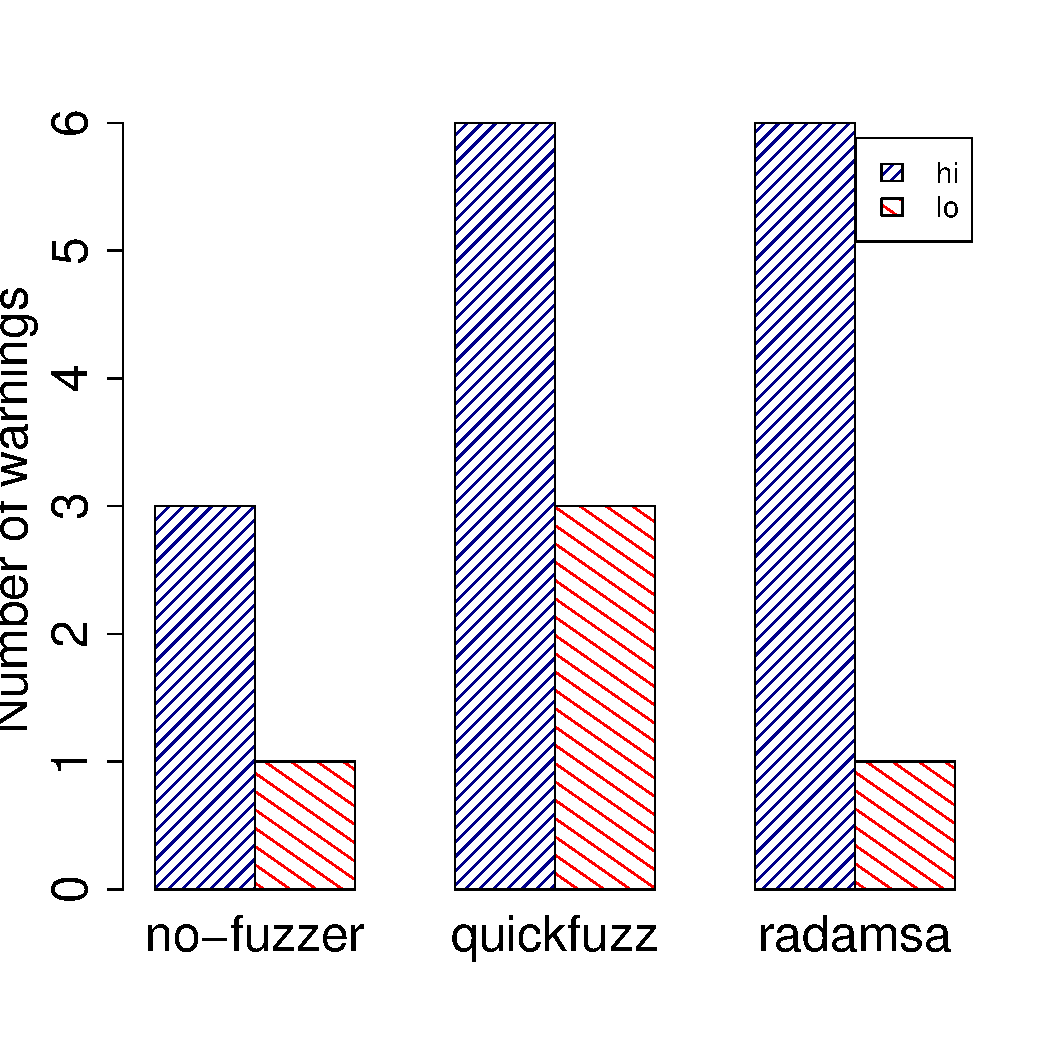
\includegraphics[trim=0 20 0 0,clip,width=0.25\textwidth]{R/barplot}  
  \caption{\label{fig:workflow}HI and LO warnings reports by each fuzzer.}
\end{figure}

\Igor{
  Para realizar nossos experimentos, tivemos que decidir qual as 
  melhores abordagens para aumentar a efetividade dos fuzzers.
  Os fuzzers mutacionais se mostraram mais eficientes em relacao
  aos fuzzers geracionais, entao focamos neste ponto.
  Utilizamos os fuzzers radamsa, QuickFuzz e \Fix{others} nas suas configuracoes
  default para realizar a mutacao em arquivos existentes.
  O fuzzer radamsa eh um fuzzer mutacional agnostico de linguagem e possui algumas
  deficiencias para a nossa infraestrutura como a falta de uma gramatica para guiar a suas mutacoes, 
  pois muitas das vezes a unica mutacao ocorre em uma palavra dentro de um comentario por exemplo.
  O fuzzer QuickFuzz tem uma gramatica JS integrada e sua mutacao ocorre de forma mais robusta que o 
  radamsa, gerando arquivos mais relevantes.
  Nossa infraestrutura usa a library Esprima\footnote{cite esprima url} para garantir que o arquivo fuzzado
  é um arquivo de teste relevante, seguindo estes requisitos:
  \begin{itemize}
    \item it contains only unicode text
    \item it is parseable (i.e., it is structurally well-formed)
    \item it does not contain engine-specific functions  
    \item it does not empty
  \end{itemize}

}

\section{Bugs Found}
\label{sec:bugs}

%% Although there are many features yet to implement in our
%% infrastructure,

\begin{table*}[h!]
  \vspace{-3ex}
%  \scriptsize
  \centering
  \caption{List of bug reports issued by our team since April,
    2018. The analysis of warnings was not uninterrupted.}
  \label{tab:bugs}
  \begin{tabular}{cccccccc}
    \toprule
    Issue\#    & Date & Fuzz & Engine  & Status  & \multicolumn{1}{c}{Url}  & Priority & Seed \\
    \midrule    
    1  & 4/12 & radamsa & Chakra   & \textbf{Fixed}  & \href{https://github.com/Microsoft/ChakraCore/issues/4978}{\#4978} & LO & WebKit \\ 
    2  & 4/12 & radamsa & Chakra   & Rejected  & \href{https://github.com/Microsoft/ChakraCore/issues/4979}{\#4979} & HI & WebKit \\
    3  & 4/14 & radamsa & JavascriptCore  & New & \href{https://bugs.webkit.org/show\_bug.cgi?id=184629}{\#184629}  & HI & WebKit    \\
    4  & 4/18 & \crossmark & JavascriptCore  & New  & \href{https://bugs.webkit.org/show\_bug.cgi?id=184749}{\#184749} & HI & JerryScript      \\
    5  & 4/23 & \crossmark & Chakra  & \textbf{Confirmed}  & \href{https://github.com/Microsoft/ChakraCore/issues/5033}{\#5033} & HI & Mozilla      \\
    6  & 4/25 & radamsa & Chakra  & \textbf{Fixed}     & \href{https://github.com/Microsoft/ChakraCore/issues/5038}{\#5038} & HI & JerryScript   \\
    7  & 4/29 & \crossmark & Chakra  & \textbf{Confirmed}   &
    \href{https://github.com/Microsoft/ChakraCore/issues/5065}{\#5065} & HI & Mozilla
    \\
    \midrule
    \multirow{2}{*}{8}  & \multirow{2}{*}{4/29} &  \multirow{2}{*}{\crossmark} & Chakra & \textbf{Confirmed} &    \href{https://github.com/Microsoft/ChakraCore/issues/5067}{\#5067} & \multirow{2}{*}{HI} & \multirow{2}{*}{Mozilla}\\
                        &  &                       &
    JavascriptCore & New &    \href{https://bugs.webkit.org/show\_bug.cgi?id=185130}{\#185130}  &   & \\
    \midrule    
    9  & 4/29 & radamsa & JavascriptCore  & New  &    \href{https://bugs.webkit.org/show\_bug.cgi?id=185127}{\#185127}  & HI  & JerryScript\\
    \midrule    
    \multirow{2}{*}{10} & \multirow{2}{*}{4/30}  & \multirow{2}{*}{radamsa} & Chakra & \textbf{Confirmed} &    \href{https://github.com/Microsoft/ChakraCore/issues/5076}{\#5076} & \multirow{2}{*}{HI} & \multirow{2}{*}{TinyJS}\\    
                        &                        &        &
    JavascriptCore & New &
    \href{https://bugs.webkit.org/show\_bug.cgi?id=185156}{\#185156} &  & 
    \\
    \midrule    
    11 & 5/02 & radamsa & JavascriptCore  & \textbf{Fixed} & \href{https://bugs.webkit.org/show\_bug.cgi?id=185197}{\#185197} & LO & Mozilla \\
    12 & 5/02 & \crossmark & JavascriptCore & New  & \href{https://bugs.webkit.org/show\_bug.cgi?id=185208}{\#185208} & HI & Mozilla \\
    13 & 5/10 & radamsa & Chakra & \textbf{Confirmed} & \href{https://github.com/Microsoft/ChakraCore/issues/5128}{\#5128} & HI & JerryScript \\
    14 & 5/17 & radamsa & Chakra & \textbf{Fixed} & \href{https://github.com/Microsoft/ChakraCore/issues/5182}{\#5182} & HI & V8\\
    15 & 5/17 & \crossmark & Chakra & \textbf{Confirmed} & \href{https://github.com/Microsoft/ChakraCore/issues/5187}{\#5187} & HI & WebKit\\
    16 & 5/21 & \crossmark & Chakra & \textbf{Confirmed} & \href{https://github.com/Microsoft/ChakraCore/issues/5203}{\#5203} & LO & Mozilla\\
    17 & 5/24 & radamsa & JavascriptCore & \textbf{Fixed}  & \href{https://bugs.webkit.org/show\_bug.cgi?id=185943}{\#185943} & HI & Webkit\\
    18 & 6/26 & radamsa & JavascriptCore & \textbf{Fixed}  & \href{https://bugs.webkit.org/show_bug.cgi?id=187042}{\#187042} & HI & JerryScript\\
    19 & 6/28 & \crossmark & Chakra & \textbf{Confirmed}  & \href{https://github.com/Microsoft/ChakraCore/issues/5388}{\#5388} & HI & WebKit\\
    20 & 7/10 & quickfuzz & JavaScriptCore & \textbf{Fixed}  & \href{https://bugs.webkit.org/show_bug.cgi?id=187520}{\#187520} & HI & JerryScript\\
    22 & 7/10 & \crossmark & Chakra & \textbf{Confirmed} & \href{https://github.com/Microsoft/ChakraCore/issues/5442}{\#5442} & HI & JerryScript\\
    21 & 7/10 & quickfuzz & Chakra & \textbf{Confirmed}  & \href{https://github.com/Microsoft/ChakraCore/issues/5443}{\#5443} & HI & JerryScript\\
    23 & 7/18 & \crossmark & Chakra & \textbf{Confirmed} & \href{https://github.com/Microsoft/ChakraCore/issues/5478}{\#5478} & HI & Mozilla\\
    24 & 7/18 & \crossmark & JavascriptCore & New & \href{https://bugs.webkit.org/show_bug.cgi?id=187777}{\#187777} & HI & JerryScript\\
   \bottomrule
  \end{tabular}
\end{table*}


This section shows results obtained with our
infrastructure. Table~\ref{tab:bugs} shows the list of bugs we
reported on issue trackers of different engines in the period of 42
days. So far, ten of the bugs we reported
were confirmed, two of which were fixed. One bug report we
submitted was rejected on the basis that the offending JS file
manifested an expected incompatibility across engine
implementations.
Note from the table that all bug
reports still waiting for confirmation are associated with the
JavaScriptCore engine (JSC). A closer look at the JSC issue tracker
showed that the triage process is very slow for that engine. 
\Igor{
The bugs reported on Chakra's bug tracker was defined as confirmed, 
however the bugs are included on a milestone for the next release
following an internal priority.
}
As of now, we did not find any new bug on SpiderMonkey and V8; 
the bugs we found were duplicates and were not reported. Finally, it is
worth noting that \Fix{11 of the 19} JS files that manifested
discrepancies were \emph{not} produced with fuzzing (column
``Fuzz''). These are test files from suites of different engines. This
observation emphasizes the importance of continuously collecting test suites from
multiple sources; today, we use test suites from seven different open
source engines, including a total of 30K test files.

\Mar{justify why we discuss these bugs} \Mar{discuss other bugs}

\vspace{1ex}\noindent\textbf{Bug \# 6.} The JS code \CodeIn{var a = \{valueOf:~function()\{return
  ``\textbackslash{}x00''\}\} assert(+a === 0)\}} 
manifested a bug in the \js{} engine Chakra.  The object
property \CodeIn{valueOf} stores a function that returns a primitive
value identifying the target object~\cite{valueof}. The original
version of this code returns an empty string whereas the version of
the code modified by the Radamsa fuzzer~\cite{radamsa} returns a string
representation of a null character (called \CodeIn{NUL} in ascii). The
unary plus expression ``\CodeIn{+a}", appearing in the assertion, is
equivalent to the abstract operation \CodeIn{ToNumber(a.valueOf())}
that converts a string to a number, otherwise the operation returns
NaN (Not a Number)\cite{unary-plus}. For this case, Chakra evaluates
the unary plus to NaN as expected, as the null character cannot be
converted. As result, the test fails as expected. Chakra, in contrast,
incorrectly converts the string to zero, making the test to pass. All
other engines fail on this test. As Table~\ref{tab:bugs} shows, the
Chakra team fixed the issue soon after we reported the problem.

\subsection{False Positives}

An example of a warning from the HI group is defined in Figure~\ref{fig:hi-priority}. 
This is a testcase from WebKit.es6 suite that it was mutate by radamsa fuzzer, the 
initial seed has in line 3 the code \CodeIn{"foo".repeat(3)} but the fuzzer changed the 
integer 3 to a big integer number. We reported this case in chakra due a core dumps that occurs
during the runtime, however this case was rejected due \CodeIn{incompatibility by design} that
this is an intentional behavior of engine that crash the process if it runs out of memory.

\begin{figure}[h!]
  \centering
  \scriptsize
  \lstset{escapeinside={@}{@},
    numbers=left,xleftmargin=1em,frame=single,framexleftmargin=0.5em,
    basicstyle=\ttfamily\scriptsize, boxpos=c,
    numberstyle=\tiny,
    morekeywords={assertEq, var, yield, in, function, 
    typeof, return, throw, new, Error, if},
  }
  \begin{lstlisting}
function test() {
  return typeof String.prototype.repeat === "function"
    && "foo".repeat(657604378) === "foofoofoo";
}
if (!test())
  throw new Error("Test failed");
  \end{lstlisting}
  \normalsize
  \caption{Warning captured as HI priority.}
  \label{fig:hi-priority}
  \end{figure}

% \subsection{LO bugs}
% 
% \Igor{For example, a bug caught by our environment and reported as LO priority was reported 
% on Chakra engine, the JS code can be found in Figure~\ref{fig:lo-priority}. In this case,
% this is a seed from Mozilla suite (\CodeIn{mozilla/non262/statements/for-in-with-assignments.js}),
% the warning was not caught by the \CodeIn{assertEq} function that compares if two arguments are equals, 
% the bug appears inside the generator function\footnote{Generators \url{https://developer.mozilla.org/en-US/docs/Web/JavaScript/Reference/Statements/function*}}
% at line 2. According to ES6 specification\footnote{ES6 YieldExpression \url{https://www.ecma-international.org/ecma-262/8.0/index.html\#prod-YieldExpression}},
% it is allowed the use of \CodeIn{yield in} in a \CodeIn{for} loop. In our infrastructure,
% only Chakra engine fails with an error output \CodeIn{SyntaxError: Syntax error}, due
% the output does not shows nothing related with assertions, we considered this one as a warning from LO group.
% Until now, the issue was confirmed and waiting for merge/closed.
% \Fix{checar ate o prazo de submissao. Essa issue esta confirmada e com commits, falta apenas o merge.}
% }
% \begin{figure}[h!]
%   \centering
%   \scriptsize
%   \lstset{escapeinside={@}{@},
%     numbers=left,xleftmargin=1em,frame=single,framexleftmargin=0.5em,
%     basicstyle=\ttfamily\scriptsize, boxpos=c,
%     numberstyle=\tiny,
%     morekeywords={assertEq, var, yield, in, function},
%   }
%   \begin{lstlisting}
% function* g1() {
%   for (var x = yield in {}) ;
% }
% var it = g1();
% assertEq(it.next().done, false);
% assertEq(it.next().done, true);
%   \end{lstlisting}
%   \normalsize
%   \caption{Bug caught by our environment as LO priority.}
%   \label{fig:lo-priority}
%   \end{figure}
  


\section{Related Work}

\Fix{The
  closest work to ours was done by Patra and Pradel~\cite{patra2016learning},
  where they evaluated their proposed language-agnostic fuzzer to find
  cross-browser HTML+JS discrepancies. This project aims at building
  and evaluating an infrastructure for differential testing of runtime
  engines, such as the JS engine or WebAssembly's. The sensible parts
  of the infrastructure are the checks of input validity (as to reduce
  waste/cost) and output correctness (as to reduce false positives).}

RFC-Directed Differential Testing of Certificate Validation in SSL/TLS Implementations...[ICSE18]

%\section*{Acknowledgment}

%\bibliographystyle{IEEEtran}
\bibliographystyle{plain}
\bibliography{references,../docs/google-research-awards-latam/tmp}

\end{document}
